\section*{Внешние данные. Табличные функции}
\addcontentsline{toc}{section}{Внешние данные. Табличные функции}
\subsection*{Чтение из Excel -- фигуры}
\addcontentsline{toc}{subsection}{Чтение из Excel -- фигуры}

\textbf{Задание:}\\
Построить фигуры, считав данные о типах фигур и их параметрах из файла ФигурыExcel.xlsx (для отрезков указаны координаты концов, для прямоугольников -- координаты левого верхнего угла).\\

\textbf{Решение:}\\
Для того, чтобы связать Excel файл с моделью, необходимо использовать блок -- файл Excel. Для загрузки была создана кнопка \textit{Load}. (Рисунок \ref{fig:excel1})
\begin{figure}[h]
	\centering 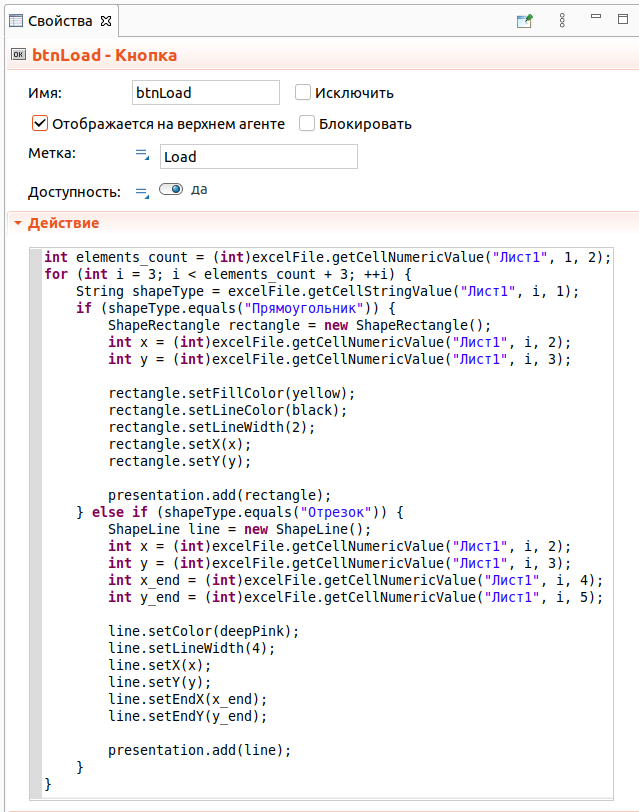
\includegraphics[scale=0.4]{excel1}
	\caption{Логика кнопки для загрузки данных из файла}
	\label{fig:excel1}
\end{figure}

\newpage

При нажатии на данную кнопку происходит отрисовка фигур заданных типов с заданными параметрами. (Рисунок \ref{fig:excel2})
\begin{figure}[h]
	\centering 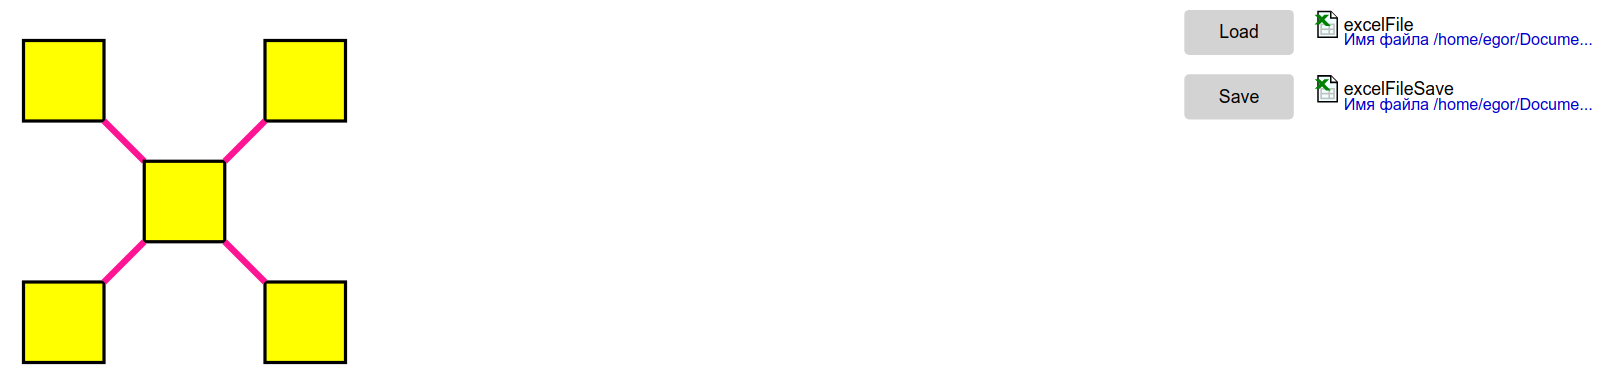
\includegraphics[scale=0.3]{excel2}
	\caption{Результат нажатия на кнопку \textit{Load}}
	\label{fig:excel2}
\end{figure}

Таким образом, по данным из excel файла нами были построены необходимые фигуры, тем самым нами был рассмотрен процесс чтения данных из excel файла.